\chapter{Related work}
\label{chap:premierchapitre}
\minitoc

%\noindent Introduction du chapitre:
%\begin{itemize}
%	\item Hypothèse: considérer les séries temporelles comme des vecteurs de données statiques
%	\item Appliquer les méthodes classiques de machine learning
%	\item NB : Faire bien attention à bien utiliser MES notations
%\end{itemize}


\fbox{  \parbox{0.9\textwidth}{
In this chapter, we recall some concepts of machine learning. First, we review the principles, the learning framework and the evaluation protocol in supervised learning. Then, we present the algorithms used in our work: $k$-Nearest Neighbors ($k$-NN) and Support Vector Machines ({\sc svm}). 
% Time series and more generally temporal data are data objects that are frequently common nowadays. By considering time series as a vector, one can use classic learning algorithms that are designed for static data. We first present a state of the art of some learning algorithms used for classification and regression. Then, we review the protocol used to learn the best fitting of the hyper-parameters of these algorithms and how we evaluate and compare the different algorithms performances.
}  }


%----------------------------------------------------------------------------
\section{Classification, Regression}

% We are going to detail now a few number of machine learning algorithms used classically to solve classification or regression problems. Other algorithms are popular nowadays such as Deep neural network, Decision tree or Relevance vector machine. We focus on $k$-Nearest Neighbors ($k$-NN) and Support Vector Machine ({\sc svm}) because these algorithms are based on the comparison of samples (time series in our case) through a distance measure, notion detailed in the next chapters.

In this section, we review some terminology used in machine learning. First, we recall the principle of machine learning. Then, we detail how to design a framework for supervised learning. After that, we present model evaluation. Finally, we review data normalization. 

\subsection{Machine learning principle}
The idea of machine learning (also known as pattern learning or pattern recognition) is to imitate with algorithms executed on computers, the ability of living beings to learn from examples. For instance, to teach a child how to read letters, we show him during a training phase, labeled examples of letters ('A', 'B', 'C', etc.) written in different styles and fonts. We don't give him a complete and analytic description of the topology of the characters but labeled examples. Then, during a testing phase, we want the child to be able to recognize and to label correctly the letters that have been seen during the training, and also to generalize to new instances \cite{Dreyfus2006}. 

Let $X=\{\textbf{x}_i,y_i\}_{i=1}^n$ be a training set of $n$ vector samples $\textbf{x}_i \in \mathbb{R}^p$ and $y_i$ their corresponding labels. The aim of supervised machine learning is to learn a relationship (model) $f$ between the samples $\textbf{x}_i$ and their labels $y_i$ based on examples \cite{Bishop2006,Dreyfus2006,Duda1973}. %This relationship can include static relationships, correlations, dynamic relationship, etc. 
After the training phase based on labeled examples $(\textbf{x}_i,y_i)$, the model $f$ has to be able to generalize on the testing phase, \textit{i.e.}, to give a correct prediction $\hat{y}_j$ for new instances $\textbf{x}_j$ that haven't been seen during the training.

When $y_i$ are class labels (\textit{e.g.}, class 'A', 'B', 'C' in the case of child's reading), learning the model $f$ is a classification problem; when $y_i$ is a continuous value (\textit{e.g.}, the energy consumption in a building), learning $f$ is a regression problem. 
% Both problems corresponds to supervised learning as $\textbf{x}_i$ and $y_i$ are known during the training phase . 
For both problems, when a part of the labels $y_i$ are known and an other part of $y_i$ is unknown during training, learning $f$ is a semi-supervised problem \cite{Zhu2007}. Note that when the labels $y_i$ are totally unknown, learning $f$ refers to a clustering problem (unsupervised learning) \cite{Jain1999,Chen1996}, out of the scope of this work.



\subsection{Model selection in supervised learning}
\label{sec:model_selection}
%\begin{itemize}
%	\item Learning framework (train, validation, test): la plupart des algorithmes requiert l'optimisation d'un hyper-paramètre. Le jeu de train permet d'apprendre les meilleurs hyper-paramètres.
%	\item Cross-validation (pourquoi on fait de la cross-validation, comment on la fait (Faire un schéma))
%\end{itemize}	
A key objective of supervised learning algorithms is to build models $f$ with good generalization capabilities, \textit{i.e.}, models $f$ that correctly predict the labels $y_j$ of new unknown samples $\textbf{x}_j$. There exists two types of errors committed by a classification or regression model $f$: training error and generalization error. \textbf{Training error} is the error on the training set and \textbf{generalization error} is the error on the testing set. A good supervised model $f$ must not only fit the training data $X$ well, it must also accurately classify records it has never seen before (test set $X_{Test}$). In other words, a good model $f$ must have low training error as well as low generalization error. This is important because a model that fits the training data too much can have a poorer generalization error than a model with a higher training error. Such a situation is known as model overfitting (Fig. \ref{fig:Overfitting}).

\begin{figure}[h!]
	\centering
	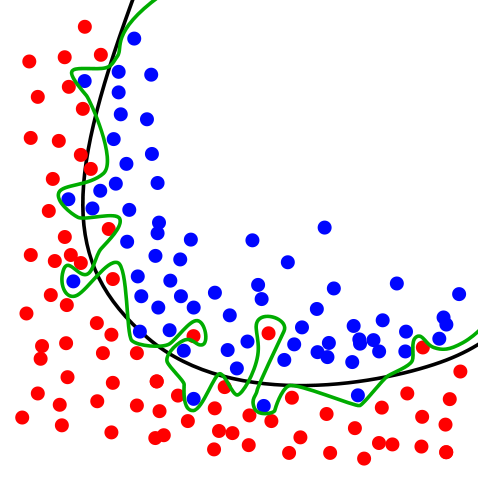
\includegraphics[width=0.4\linewidth]{images/Overfitting}
	\caption{An example of overfitting in the case of classification. The objective is to separate blue points from red points. Black line shows a classifier $f_1$ with low complexity where as green line illustrates a classifier $f_2$ with high complexity. On training examples (blue and red points), the model $f_2$ separates all the classes perfectly but may lead to poor generalization on new unseen examples. Model $f_1$ is often preferred.}
	\label{fig:Overfitting}
\end{figure}

In most cases, learning algorithms require to tune some hyper-parameters. A first approach could consist in trying all the possible combinations of hyper-parameters values and keep the one with the lowest training error. However, as discussed above, the model with the lowest training error is not always the one with the best generalization error.  To avoid overfitting, the training set can be divided into 2 sets: a learning and a validation set. Suppose we have two hyper-parameters to tune: $C$ and $\gamma$. We make a grid search for each combination $(C,\gamma)$ of the hyper-parameters, that is in this case a 2-dimensional grid (Fig. \ref{fig:GridSearch}). For each combination (a cell of the grid), the model is learnt on the learning set and evaluated on the validation set. At the end, the model with the lowest error on the validation set is retained. This process is referred as the model selection. 

\begin{figure}[h!]
	\centering
	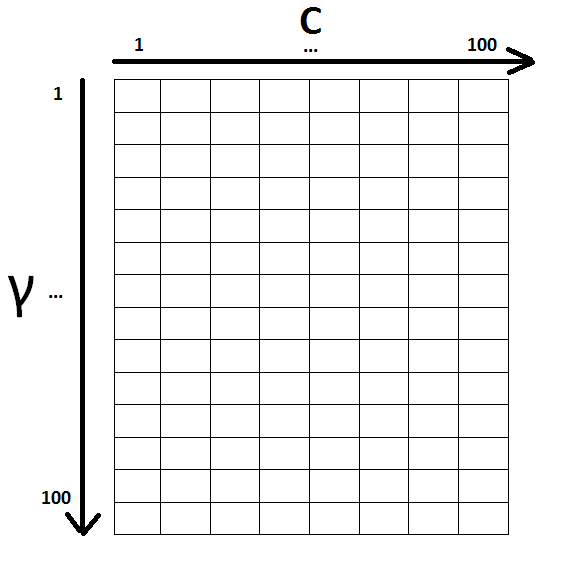
\includegraphics[width=0.4\linewidth]{images/GridSearch}
	\caption{Example of a 2 dimensional grid search for parameters $C$ and $\gamma$. It defines a grid where each cell of the grid contains a combination ($C$, $\gamma$). Each combination is used to learn the model and is evaluated on the validation set.}
	\label{fig:GridSearch}
\end{figure}

\begin{figure}[h!]
	\centering
	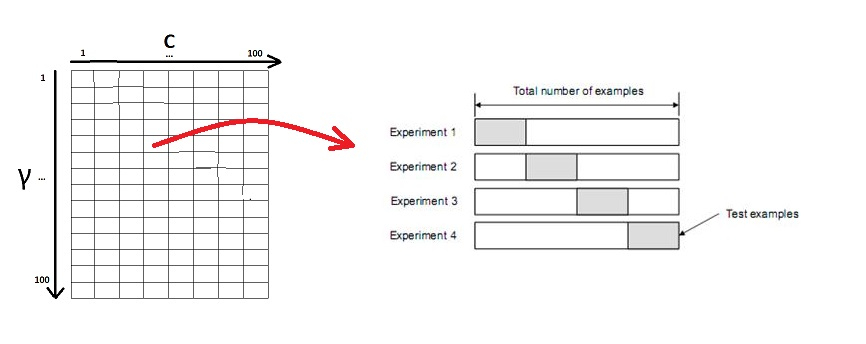
\includegraphics[width=1\linewidth]{Cross_validation2}
	\caption{$v$-fold Cross-validation for one combination of parameters. For each of $v$ experiments, use $v-1$ folds for training and a different fold for Testing, then the training error for this combination of parameter is the mean of all testing errors. This procedure is illustrated for $v=4$.}
	\label{fig:Cross_validation}
\end{figure}

An alternative is cross-validation with $v$ folds, illustrated in Fig. \ref{fig:Cross_validation}. In this approach, we partition the training data into $v$ equal-sized subsets. The objective is to evaluate the error for each combination of hyper-parameters. For each run, one fold is chosen for validation, while the $v-1$ remaining folds are used as the learning set. We repeat the process for each fold, thus $v$ times. Each fold gives one validation error and thus we obtain $v$ errors. The total error for the current combination of hyper-parameters is obtained by summing up the errors for all $v$ folds. When $v=n$, the size of training set, this approach is called leave-one-out or Jackknife. Each test set contains only one sample. The advantage is that as much data as possible are used for training. Moreover, the validation sets are exclusive and they cover the entire data set. The drawback is that it is computationally expensive to repeat the procedure $n$ times. Furthermore, since each validation set contains only one record, the variance of the estimated performance metric is usually high. This procedure is often used when $n$, the size training set, is small. There exists other methods such as sub-sampling or bootstraps \cite{Duda1973,Dreyfus2006}. We only use cross-validation in our experiments.

\noindent To sum up, Fig. \ref{fig:LearningFramework} shows a general approach for solving machine learning problems. In general, a dataset can be divided into 3 sub-datasets (illustrated in Fig. \ref{fig:Dataset}):
\begin{itemize}
	\item A \textbf{training set} $X=\{\textbf{x}_i,y_i\}_{i=1}^n$, which consists of $n$ samples $\textbf{x}_i$ whose labels $y_i$ are known. The training set is used to build the supervised model $f$. When the learning algorithm requires some hyper-parameters to be tuned, there exists a risk of model overfitting. To avoid such risks, the training set $X$ has to be divided into two subsets :
	\begin{itemize}
		\item A \textbf{learning set} which is used to build the supervised model $f$ for each value of the hyper-parameters.
		\item A \textbf{validation set} which is used to evaluate the supervised model $f$ for each value of the hyper-parameter. The model $f$ with the lowest error on the validation set is kept, thus ensuring that it has the best generalization abilities.
	\end{itemize}
	\item A \textbf{test set} $X_{Test}=\{\textbf{x}_j,y_j\}_{j=1}^m$, which consists of $m$ samples $\textbf{x}_j$ whose labels $y_j$ are also known but are not used during the training step. The model $f$ is applied to predict the label $\hat{y_j}$ of samples $\textbf{x}_j$ to evaluate the performance of the learnt model by comparing $\hat{y_j}$ and $y_j$. 
	\item An \textbf{operational set} $X_{op}=\{\textbf{x}_l,y_l\}_{l=1}^L$, which consists of $L$ samples $\textbf{x}_l$ whose labels $y_l$ are totally unknown. The operational set is in general a new dataset on which the learnt algorithm is applied. 
\end{itemize}


\begin{figure}[h!]
	\centering
	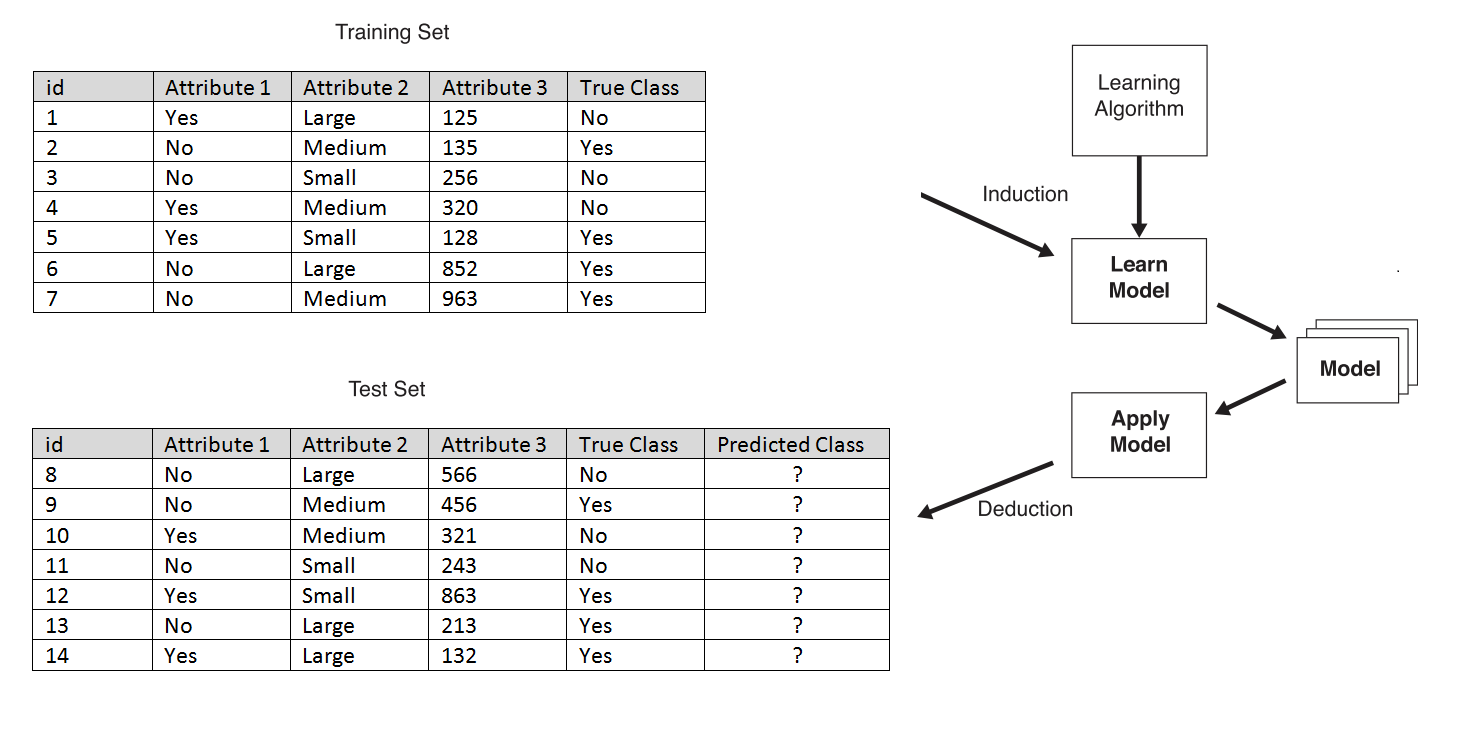
\includegraphics[width=1\linewidth]{images/LearningFramework}
	\caption{General framework for building a supervised (classification/regression) model. Example with 3 features and 2 classes ('Yes' and 'No').}
	\label{fig:LearningFramework}
\end{figure}

\begin{figure}[h!]
	\centering
	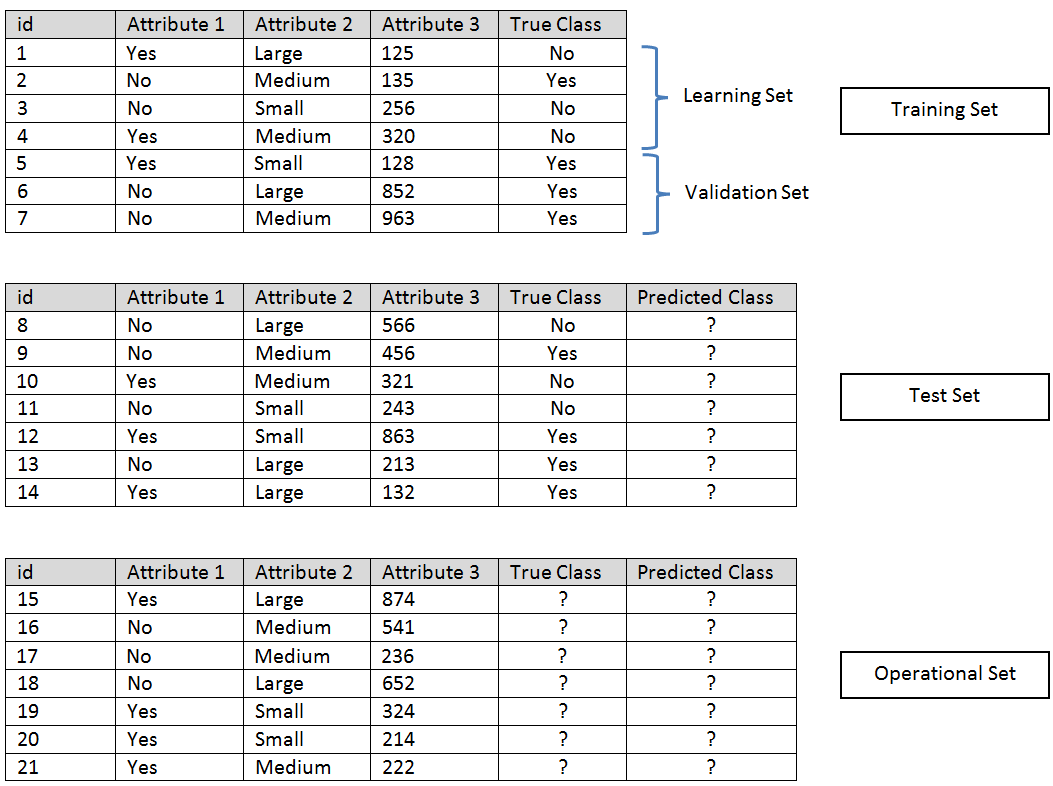
\includegraphics[width=0.9\linewidth]{images/Dataset}
	\caption{Division of a dataset into 3 datasets: training, test and operational.}
	\label{fig:Dataset}
\end{figure}

%\mycomment[MR]{refaire cette partie là} First, a training set $X=\{(\textbf{x}_i,y_i)\}_{i=1}^n$ consisting of $m$ samples $\textbf{x}_i$ whose labels $y_i$ are known is provided. The training set is used to build the supervised model $f$. Then, the model is applied to the test set $X_{Test}=\{(\textbf{x}_j,y_j)\}_{j=1}^m$, which consists of samples $\textbf{x}_j$ with unknown labels $y_j$. The test is used to evaluate the performance of the learnt model. 



\newpage
\subsection{Model evaluation}
%\begin{itemize}
%	\item Classification Error et test de significativité
%	\item Regression Error
%\end{itemize}

As seen in the previous section, model selection is inherently based on the ability to quantify its error on the training and validation sets. In this section, we recall how this error is computed for classification and regression problems.

\subsubsection{Classification evaluation}
\label{sec:ClassificationEvaluation}
The performance of a classification model is based on the counts of test samples $\textbf{x}_j$ correctly and incorrectly predicted by the model $f$. These counts are tabulated in a table called the confusion matrix. Table \ref{fig:ConfusionMatrix} illustrates the concept for a binary classification problem. Each cell $g_{ij}$ of the table stands for the number of samples from class $i$ predicted to be of class $j$. Based on this matrix, the number of correct predictions made by the model is $\sum_{i=1}^C g_{ii}$, where $C$ is the number of classes. % Equivalently, the ratio of incorrect predictions is $1-\sum_{i=1}^C g_{ii}$.

\begin{table}[h!]
	\centering
	\begin{tabular}{|c|c|c|c|}
		\hline      &  & \multicolumn{2}{c|} {Predicted class } \\ 
		\cline{3-4} &  & Class = 1 & Class = 0  \\ 
		\hline  \multirow{2}{*}{Actual Class } & Class = 1  & $g_{11}$ & $g_{10}$ \\ 
		\cline{2-4}  & Class = 0  & $g_{01}$ & $g_{00}$ \\ 
		\hline 
	\end{tabular}
	\caption{Confusion matrix for a 2-class problem.} 
	\label{fig:ConfusionMatrix}
\end{table}

\noindent For binary classification problems, $g_{11}$ is the number of true positives, $g_{10}$ is the number of false negatives, $g_{01}$ is the number of false positives and $g_{00}$ is the number of true negatives.

To summarize the information, it generally more convenient to use performance metrics such as the classification accuracy ($Acc$) or error rate ($Err$). This allows to compare several models with a single number. Note that $Err = 1-Acc$.
\begin{align}
Acc & = \frac{\text{Number of correct predictions}}{\text{Total number of predictions}} = \frac{\sum\limits_{i=1}^{C} g_{ii}}{\sum\limits_{i,j=1}^{C} g_{ij}} \\
Err & = \frac{\text{Number of wrong predictions}}{\text{Total number of predictions}} = \frac{\sum\limits_{i,j=1, i \neq j}^{C} g_{ij}}{\sum\limits_{i,j=1}^{C} g_{ij}}
\end{align}

Using these performance metrics allows to compare the performance of different classifiers $f$. It allows to determine in particular whether one learning algorithm outperforms another on a particular learning task on a given test dataset $X_{Test}$. However, depending on the size of the test dataset, the difference in error rate $Err$ between two classifiers may not be statistically significant. Snedecor \& Cochran proposed in 1989 a statistical test based on measuring the difference between two learning algorithms \cite{Cochran1977}. It has been used by many researchers \cite{Dietterich1997,Dietterich1995}.

Let consider 2 classifiers $f_A$ and $f_B$. We test these classifiers on the test set $X_{Test}$ and denote $p_A$ and $p_B$ their respective error rates. The intuition of this statistical test is that when algorithm A classifies an example $\textbf{x}_j$ from the test set $X_{Test}$, the probability of misclassification is $p_A$. Thus, the number $m_A$ (resp. $m_B$) of misclassification of $m$ test examples made by classifier $f_A$ (resp. $f_B$) is a binomial random variable with mean $mp_A$ and variance $p_A(1-p_A)m$. The binomial distribution can be approximated by a normal distribution when $m$ has a reasonable value (Law of large numbers). The difference between two independent normally distributed random variables is also normally distributed with a mean $m(p_A-p_B)$. Thus, the quantity $m_A-m_B$ is a normally distributed random variable. Under the null hypothesis (the two algorithm should have the same error rate), this will have a mean of zero and a standard error $se$ of:
\begin{equation}
se = \sqrt{\frac{2p(1-p)}{m}}
\end{equation}
\noindent where $p=\frac{p_A+p_B}{2}$ is the average of the two error probabilities. From this analysis, we obtain the statistic:
\begin{equation}
z=\frac{p_A-p_B}{\sqrt{2p(1-p)/m}}
\end{equation}
\noindent which has (approximatively) a standard normal distribution. We can reject the null hypothesis if $|z| > Z_{0.975} = 1.96$ (for a 2-sided test with probability of incorrectly rejecting the null hypothesis of 0.05).


\subsubsection{Regression evaluation}
As the concept of classes is restricted to classification problems, the performance of a regression model $f$ is based on metrics that measure the difference between the predicted label $\hat{y}_j$ and the known label $y_j$. The Mean Absolute Error function ($MAE$) computes the mean absolute error, a risk metric corresponding to the expected value of the absolute error loss or $L_1$-norm loss.

\begin{equation}
MAE = \frac{1}{m} \sum_{j=1}^m|\hat{y}_j-y_j|
\end{equation}

A commonly used performance metrics is the Root Mean Squared Error function ($RMSE$) that computes the root of the mean square error, a risk metric corresponding to the expected value of the squared (quadratic) error loss.

\begin{equation}
RMSE = \sqrt{\frac{1}{m} \sum_{j=1}^m(\hat{y}_j-y_j)^2}
\end{equation}

Many works rely on the $R^2$ function, the coefficient of determination. It provides a measure of how well future samples are likely to be predicted by the model \footnote{\url{http://scikit-learn.org/stable/modules/model_evaluation.html}}. It can also be interpreted as a measure of how the model $f$ is better than a constant model \todo{ref sylvain?}. 

\begin{equation}
R^2 = 1- \frac{\sum_{j=1}^m (\hat{y}_j-y_j)^2}{\sum_{j=1}^m (\bar{y}-y_j)^2}
\end{equation}

\noindent where $\bar{y} = \sum_{j=1}^m y_j$ is the mean over the known labels $y_j$.


\subsection{Data normalization}
\label{sec:data_normalization}
Real dataset are often subjected to noise or uneven scaling. Before applying any learning protocol, it is often necessary to pre-process the data: data scaling, data filtering (\textit{e.g.}, de-noising), outlier removal, etc. We focus on data normalization (data scaling) in our work.

Part 2 of Sarle's Neural Networks FAQ (1997) \footnote{\url{http://www.faqs.org/faqs/ai-faq/neural-nets/}} explains the importance of data normalization for neural networks but they can be applied to any learning algorithms. The main advantage of normalization is to avoid attributes in greater numeric ranges to dominate those in smaller numeric ranges. Another advantage is to avoid numerical difficulties during the calculation. For example, in the case of Support Vector Machine ({\sc svm}), because kernel values usually depend on the inner products of feature vectors, \textit{i.e.} the linear kernel and the polynomial kernel, large attribute values might cause numerical problems \cite{Hsu2008}. 

In most cases, it is recommended to scale each attribute to the range [-1; +1] or [0; 1]. Many normalization methods have been proposed such as Min/Max normalization, Z-normalization or normalization of the log distribution \todo{références normalization}. Let $X=\{\textbf{x}_i,y_i\}_{i=1}^n$ be a training set, $\textbf{x}_i$ being a sample described by $p$ features $x_1, \ldots, x_p$. We define $\mu_j$ and $\sigma_j$ as the mean and the standard deviation of a variable $x_j$, applying the Z-normalized variable $x^{norm}_j$ is given by:
\begin{equation}
x^{norm}_j = \frac{x_j-\mu_j}{\sigma_j}
\end{equation}
%Note that the underlying assumption supposes that the variable $x_j$ is normally distributed: data evolves between $[-\infty;+\infty]$ and are coming from a Gaussian process. In some cases, the data are skewed such as monetary amounts or incomes. These data are sometimes log-normally distributed, \textit{e.g.}, the log of the data is normally distributed (Fig. \ref{fig:SkewedData}). The underlying idea is to take the log of the data ($x^{ln}_j$) to restore the symmetry, and then, to apply a Z-normalization of this transformation:
%\begin{align}
%x^{ln}_j 		& = \ln(x_j); \\
%x^{ln,norm}_j & = \frac{x^{ln}_j-\mu^{ln}_j}{\sigma^{ln}_j} \\
%x^{norm}_j 	& = \exp(x^{ln,norm}_j)
%\end{align}
%
%\noindent where $\ln$ denotes the Natural Logarithm function, $\mu^{ln}_j$ and $\sigma^{ln}_j$ the mean and the standard deviation of a variable $x^{ln}_j$.
%
%\begin{figure}
%	\centering
%	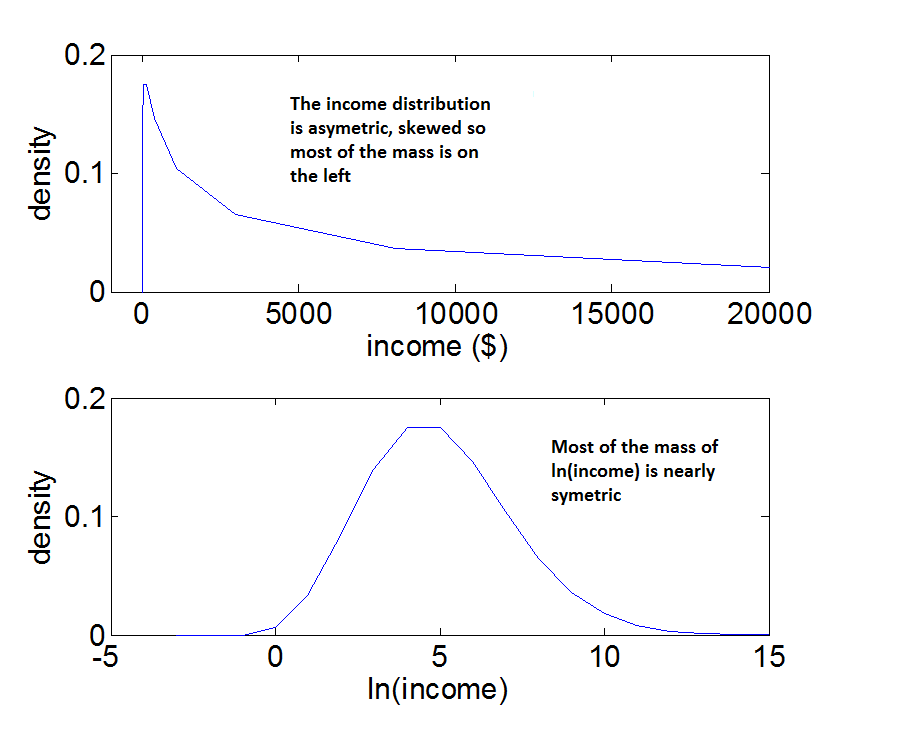
\includegraphics[width=0.6\linewidth]{images/SkewedData2}
%	\caption{A nearly log-normal distribution, and its log transform \protect\footnotemark}
%	\label{fig:SkewedData}
%\end{figure}
%\footnotetext{source: \url{http://www.r-statistics.com/2013/05/log-transformations-for-skewed-and-wide-distributions-from-practical-data-science-with-r/}}

Finally, we recall some precautions to the practitioner in the learning protocol, experimented by Hsu \& al. in the context of {\sc svm} \cite{Hsu2008}. First, training and testing data must be scaled using the same method. Second, training and testing data must not be scaled separately. Third, the whole dataset must not be scaled together at the same time. These often leads to poorer results. A proper way to do normalization is to scale the training data, store the parameters of the normalization (\textit{e.g.} $\mu_i$ and $\sigma_i$ for Z-normalization), then apply the same normalization to the testing data. 


%------------------------------------------------------------------------------
\newpage
\section{Machine learning algorithms}

\mycomment[AD]{dit d'enlever 1ère phrase mais Michèle dit de garder}Many algorithms have been proposed in the context of supervised learning, such as Deep Neural Networks, Decision Trees or Relevance Vector Machines ({\sc rvm}). Our proposition relies on both results from Support Vector Machines ({\sc svm}) in the context of $k$-Nearest Neighbors ($k$-NN) classification. We limit the section to present these two algorithms. 
% We focus on $k$-Nearest Neighbors ($k$-NN) and Support Vector Machine ({\sc svm}). % The interest of these two is that they are based on the comparison of samples (time series in our case) through a distance measure, notion detailed in the next chapters.  

% We are going to detail now a few number of machine learning algorithms used classically to solve classification or regression problems. Other algorithms are popular nowadays such as Deep neural network, Decision tree or Relevance vector machine. We focus on $k$-Nearest Neighbors ($k$-NN) and Support Vector Machine ({\sc svm}) because these algorithms are based on the comparison of samples (time series in our case) through a distance measure, notion detailed in the next chapters.

\subsection{$k$-Nearest Neighbors ($k$-NN) classifier}
\label{sec:kNN}
%\begin{itemize}
%	\item Donner l'intuition
%	\item Formaliser le problème en tant que problème d'optimisation
%	\item Présenter les extensions (kNN pondéré), extension à la régression
%	\item Soulever le fait que la résolution du problème fait intervenir une notion de distance entre les individus (time series)	
%	\item Donner les arguments qui permettent de dire pourquoi utiliser un 1-NN permet de faire une évaluation de métriques (Ding)
%\end{itemize}

\mycomment[AR]{Ahlame trouve que ce n'est pas clair. A refaire}A simple approach to classify samples is to consider that "close" samples have a great probability to belong to the same class. Given a test sample $\textbf{x}_j$, one can use the class $y_i$ of its nearest neighbor $\textbf{x}_i$ in the training set in order to predict its labels: $\hat{y}_j=y_i$. \\
\indent More generally, we can consider the $k$ nearest neighbors of $\textbf{x}_j$. The class $y_j$ of a test sample $\textbf{x}_j$ is assigned with a voting scheme among them, \textit{i.e.}, using the majority of the class of nearest neighbors. This algorithm is referred as the $k$-Nearest Neighbors algorithm ($k$-NN) 
\cite{Silverman1989,Cover1967b}. Fig. \ref{fig:kNN_example} illustrates the concept for a neighborhood of $k=3$ and $k=5$.

\begin{figure}[h!]
\centering
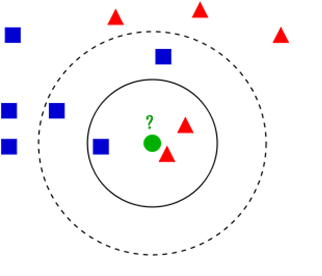
\includegraphics[width=0.40\linewidth]{images/kNN_example}
\caption{Example of $k$-NN classification. The test sample (green circle) is classified either to the first class (red stars) or to the second class (blue triangles). If $k = 3$ (solid line circle) it is assigned to the second class because there are 2 triangles and only 1 star inside the inner circle. If $k = 5$ (dashed line circle) it is assigned to the first class (3 stars vs. 2 triangles inside the outer circle).}
\label{fig:kNN_example}
\end{figure}

\indent In the $k$-NN algorithm, the notion of "closeness" between samples $\textbf{x}_i$ is based on the computation of a metric \footnote{A clarification of the terms metric, distance, dissimilarity, etc. will be given in Chapter \ref{sec:Chapter_metrics}. For now, we refer all of them as metrics.} $D$. For static data, frequently used metrics are the Euclidean distance, the Minkowski distance or the Mahalanobis distance. Considering a training set $X$ of $n$ samples, solving the 1-NN classification problem is equivalent to solve the following optimization problem: for a new sample $\textbf{x}_j$, $\forall i \in \{1...n\}$,
\begin{equation}
y_j = y_{i^*}
\end{equation}
where $i^*={\underset{i \in \{1...n\}}{\argmin}   D(\textbf{x}_i,\textbf{x}_j)}$.

The $k$-NN algorithm can be extended to estimate continous labels (regression problems). The procedure is similar. The label $y_j$ is defined as :
\begin{equation}
y_j = \frac{1}{k}\sum_{i=1}^{k} y_{i}
\end{equation}
where $i$ corresponds to the index of the $k$-nearest neighbors \cite{Altman1992}. There exists other variants of the $k$-NN algorithms. In a weighed $k$-NN, the approach consists in weighting the $k$-NN decision by assigning to each neighbor $\textbf{x}_i$ from an unknown sample $\textbf{x}_j$, a weight $w_i$ defined as a function of the distance $D(\textbf{x}_i, \textbf{x}_j)$ \cite{Dudani1976}. To cope with uncertainty or imprecision in the labeling of the training data $\textbf{x}_i$, other authors propose in a fuzzy $k$-NN to determine the membership degree in each class of an unseen sample $\textbf{x}_j$ by combining the memberships of its neighbors \cite{Keller1985}. \mycomment[AD]{Expliquer d'avantage} Denoeux propose a framework based on Dempster-Shafer theory where the $k$-NN rule takes into account the non-representativity of training data, the weighting rule and uncertainty in the labeling \cite{Denoeux1995}.

% in weighting each neighbors labels $y_{i}$ by a factor equal to the inverse of the distance $\frac{1}{D(\textbf{x}_i, \textbf{x}_j)}$ \cite{Dudani1976}. To cope with uncertainty or imprecision in the labelling of the training data, some authors propose in a fuzzy $k$-NN to determine the membership degree of an unseen pattern in each class by combining the memberships of its neighbors. assign a degree of membership of a training vector $\textbf{x}_i$ memberships of samples $\textbf{x}_j$ to classes. in a fuzzy $k$-NN, the idea is to assign memberships of samples $\textbf{x}_j$ to classes. The class membership is a function of the sample’s distance $D(\textbf{x}_i, \textbf{x}_j)$ from its $k$-NN training samples\todo{[biblio fuzzy kNN]}; in a credibilist $k$-NN\mycomment[MR]{+ $k$-NN crédibiliste} \cite{Denoeux1995}

Despite its simplicity, the $k$-NN algorithm has been shown to be successful on time series classification problems \cite{Belongie2002,Xi2006a,Ding2008}. 
%presents many advantages and
% \mycomment[AD]{Ahlame trouve que le discours s'éloigne et on devrait supprimer jusqu'à la fin des avantages}One main advantage is that a 1-NN classifier can be used to evaluate and compare the efficiency of different metrics \cite{Ding2008}. First, the underlying metric is critical in the performance of the 1-NN classifier \cite{Tan2005b}. Thus, the accuracy of the 1-NN classifier directly reflects the effectiveness of the metric. Second, 1-NN classifier is easy to implement and doesn't need to learn any hyper-parameters, which make it straightforward for anyone to reproduce results. All of this advantages allows one who want to evaluate a benchmark of metrics. Other methods to compare metrics exists such as clustering with small data sets which are not statistically significant, or compare the compactness of the metric \cite{Morse2007,Vlachos2006}. The 1-NN algorithm will be used in our experiments to compare the performances different metrics used for time series.
However, the $k$-NN algorithm presents some disadvantages, mainly due to its computational complexity, both in memory space (storage of the training samples $\textbf{x}_i$) and time (search of the neighbors) \cite{Duda1973}. Suppose that we have $n$ labeled training samples in $p$ dimensions, and find the closest neighbors to a test sample $\textbf{x}_j$ ($k = 1$). In the most simple approach, we look at each stored samples $\textbf{x}_i$ ($i=1...n$) one by one, calculate its distance to $\textbf{x}_j$ (D($\textbf{x}_i$,$\textbf{x}_j$)) and retain the index of the current closest one. For the standard Euclidean distance, each metric computation is $O(p)$ and thus the search is $O(pn)$. Finally, note that using standard metrics (such as the Euclidean distance) in the $k$-NN relies on all $p$ dimensions in its computation and thus assumes that all dimensions have the same effect on the metric. This assumption may be wrong and can impact the classification performances. 
%The importance of defining adapted metrics for time series will be discussed in Chapter \ref{sec:Chapter_metrics}.


% \textcolor{red}{Accuracy evaluation answers one of the most important questions about a similarity measure: why is this a good measure for describing the (dis)similarity between time series? Surprisingly, we found that accuracy evaluation is usually insufficient in existing literature: it has been either based on subjective evaluation, \textit{e.g.}, [4, 9], or using clustering with small data sets which are not statistically significant, \textit{e.g.}, [31, 40]. In this work, we use an objective evaluation method recently proposed [25]. The idea is to use a one nearest neighbor (1NN) classifier [17, 32] on la- belled data to evaluate the efficacy of the distance measure used. Specifically, each time series has a correct class label, and the classifier tries to predict the label as that of its nearest neighbor in the training set. There are several advantages with this approach. First, it is well known that the underlying distance metric is critical to the performance of 1NN classifier [32], hence, the accuracy of the 1NN classifier directly reflects the effectiveness of the similarity measure. Second, the 1NN classifier is straightforward to implement and is parameter free, which makes it easy for anyone to reproduce our results. Third, it has been proved that the error ratio of 1NN classifier is at most twice the Bayes error ratio [36]. Finally, we note that while there have been attempts to classify time series with decision trees, neural networks, Bayesian networks, supporting vector machines etc., the best published results (by a large margin) come from simple nearest neighbor methods [42]}

% Cons of the kNN
%Curse of Dimensionality
%* Distance usually relates to all the attributes and assumes all
%of them have the same effects on distance
%* The similarity metrics do not consider the relation of
%attributes which result in inaccurate distance and then impact
%on classification precision. Wrong classification due to
%presence of many irrelevant irrelevant attributes attributes is often termed as the
%curse of dimensionality
%* For example: Each instance is described by 20 attributes out
%of which only 2 are relevant in determining the classification
%of the target function. In this case, instances that have
%identical values for the 2 relevant attributes may
%nevertheless be distant from one another in the 20
%dimensional instance space
%(http://www.csee.umbc.edu/~tinoosh/cmpe650/slides/K_Nearest_Neighbor_Algorithm.pdf)


\subsection{Support Vector Machine ({\sc svm}) algorithm}
%\begin{itemize}
%	\item Présenter le principe général des {\sc svm} en commençant par l'intuition.
%	\item Forme primale: donner la formulation primale du problème d'optimisation
%	\item Forme duale: montrer commencer passer de la forme primal à la forme dual.
%	\item A partir de la forme duale, passer au kernel
%	\item Finir par la complexité du {\sc svm} en apprentissage ($o(N^3p)$) et en test (limités aux nombres de support vectors) et les interprétations des supports vectors.
%	\item Expliquer la modification du problème initiale avec une régularisation $L_1$ sur le terme de régularisation et nous permet d'avoir une solution sparse (donner 1 cas où la solution sparse est meilleur).
%	\item Expliquer que dans le cadre de données non-balancées, il faut ajouter des termes pour rebalancer l'équation du {\sc svm}
%\end{itemize}

Support Vector Machine ({\sc svm}) is a classification method introduced in 1992 by Boser, Guyon, and Vapnik \cite{Boser1992,Cortes1995} to solve at first linearly separable problems. The {\sc svm} classifier has demonstrated high accuracy, ability to deal with high-dimensional data, good generalization properties and interpretation for various applications from recognizing handwritten digits, to face identification, text categorization, bioinformatics and database marketing \cite{Wang2002,Yang1999,Heisele2001,Sadri2003,Campbell2011}. {\sc svm}s belong to the category of kernel methods, algorithms that depends on the data only through dot-products \cite{Schlkopf2013}. It allows thus to solve non-linear problems. This section gives a brief overview of the mathematical key points and interpretation of the method. For more informations, the reader can consult \cite{Schlkopf2013,Campbell2011,Cortes1995}.

We first present an intuition of maximum margin concept. We give the primal formulation of the {\sc svm} optimization problem. Then, by transforming the latter formulation into its dual form, the kernel trick can be applied to learn non-linear classifiers. Finally, we detail how we can interpret the obtained coefficients and how {\sc svm}s can be extended for regression problems.



\subsubsection{Intuition}
\mycomment[AD]{Mettre dans les figures des + et - pour les classes}Let $\{\textbf{x}_i,y_i\}_{i=1}^n$ be a set of $n$ samples $\textbf{x}_i \in \mathbb{R}^p$ and their labels $y_i= \pm 1$ (2 class-problem). The objective is to learn a hyperplane, whose equation is $\textbf{w}^T \textbf{x} + b = 0$, that can separate samples of class +1 from the ones of class -1. When the problem is linearly separable such as in Fig. \ref{fig:Plusieurs_separatrice_lineaire}, there exists an infinite number of valid hyperplanes. 

\begin{figure}[h!]
\centering
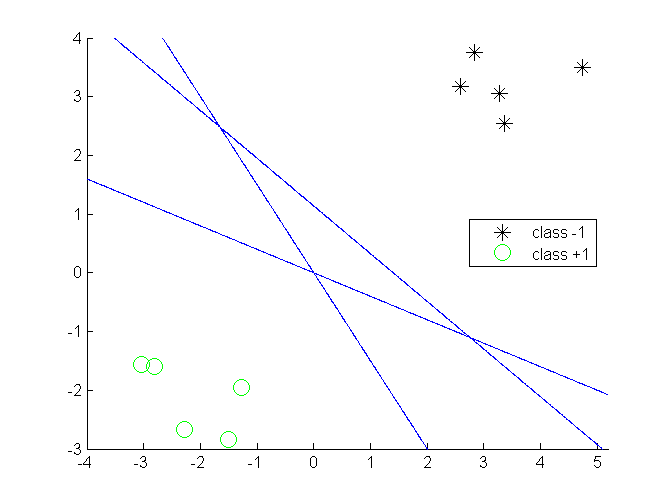
\includegraphics[width=0.5\linewidth]{images/Plusieurs_separatrice_lineaire2}
\caption{Example of linear classifiers in a 2-dimensional classification problem. For a set of points of classes +1 and -1 that are linearly separable, there exists an infinite number of separating hyperplanes corresponding to $\textbf{w}^T\textbf{x} + b = 0.$ }
\label{fig:Plusieurs_separatrice_lineaire}
\end{figure}

\noindent Vapnik \& al. \cite{Cortes1995} propose to choose the separating hyperplane that maximizes the margin, \textit{e.g.} the hyperplane that leaves as much distance as possible between the hyperplane and the closest samples $\textbf{x}_i$ of each class, called the support vectors. This distance is equal to $\frac{1}{||\textbf{w}||_2}$. We denote $||\textbf{w}||_2$, the $L_2$-norm of the vector $\textbf{w}$ and $||\textbf{w}||_1$ the $L_1$-norm of $\textbf{w}$:
\begin{align}
	||\textbf{w}||_2 & = \sqrt{\textbf{w}^T \textbf{w}} = \sqrt{\sum\limits_{h=1}^{p} w_h^2}\\
	||\textbf{w}||_1 & = \sum\limits_{h=1}^{p} |w_h|
\end{align}
\noindent where $\textbf{w} = [w_1, \ldots, w_p]^T$ denotes the weight vector. \\
The two hyperplanes passing through the support vectors of each class are referred as the canonical hyperplanes, and the region between the canonical hyperplanes is called the margin band (Fig. \ref{fig:Separatrice_lineaire_avec_marges}). From this, for a binary classification problem, to classify a new sample $\textbf{x}_j$, the decision function is:
\begin{equation}
f(\textbf{x}_j) = sign(\textbf{w}^T \textbf{x}_j + b) \label{eq:decision_function}
\end{equation}

\begin{figure}
\centering
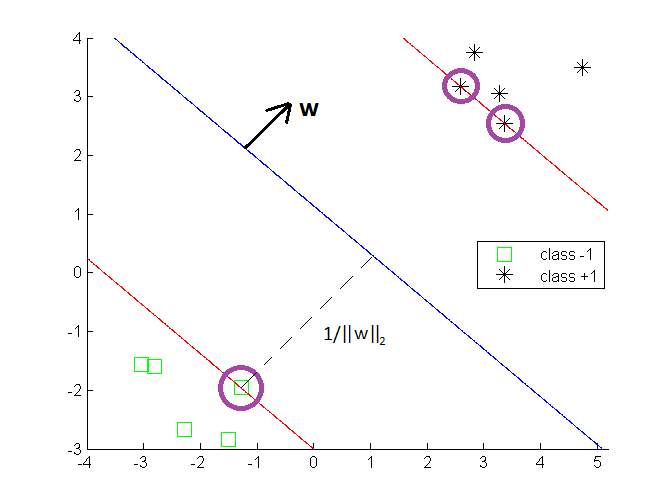
\includegraphics[width=0.6\linewidth]{images/Separatrice_lineaire_avec_marges2}
\caption{The argument inside the decision function of a classifier is $\textbf{w}^T\textbf{x} + b$. The separating hyperplane corresponding to $\textbf{w}^T\textbf{x} + b = 0$ is shown as a line in this 2-dimensional plot. This hyperplane separates the two classes of data with points on one side labeled $y_i = +1$ ($\textbf{w}^T\textbf{x}_i + b \geq 0$) and points on the other side labeled $y_i=-1$ ($\textbf{w}^T\textbf{x}_i + b < 0$). Support vectors are circled in purple and lies on the hyperplanes $\textbf{w}^T\textbf{x} + b = +1$ and $\textbf{w}^T\textbf{x} + b = -1$}
\label{fig:Separatrice_lineaire_avec_marges}
\end{figure}

% \missingfigure{Make a figure with many hyperplans. Put the one that maximize the hyperplan between the support vectors. Example of caption: }



\subsubsection{Primal formulation}
Finding $\textbf{w}$ and $b$ by maximizing the margin $\frac{1}{||\textbf{w}||_2}$ is equivalent to minimizing the norm of $\textbf{w}$ such that all samples from the training set are correctly classified:
	\begin{align}
		& \argmin_{\textbf{w},b} \frac{1}{2} ||\textbf{w}||_2^2 \label{eq:objectiveSVM}\\
		& \textbf{s.t. } y_i(\textbf{w} ^T\textbf{x}_i+b) \geq 1 \label{eq:constraintsSVM}
	\end{align}
This is a constrained optimization problem in which we minimize an objective function (Eq. \ref{eq:objectiveSVM}) subject to constraints (Eq. \ref{eq:constraintsSVM}). This formulation is referred as the primal hard margin problem. When the problem is not linearly separable, slack variables $\xi_i \geq 0$ are introduced to relax the optimization problem:
	\begin{align}
	& \argmin_{\textbf{w},b, \xi}  
	\left( 
	\overbrace{\vphantom{\sum_{i=1}^n \xi_i}
		\frac{1}{2}||\textbf{w}||^2_2}^{Regularization}
	+ C \overbrace{\sum\limits_{i=1}^{n}\xi_i}^{Loss} \right) 
	\label{eq:objectiveSVM2}\\
	& \textbf{s.t. } y_i(\textbf{w}^T\textbf{x}_i+b) \geq 1 -\xi_i \label{eq:constraintsSVM2} \\
	&  \xi_i \geq 0 \label{eq:constraintsSVM20}
	\end{align}
\noindent where $C > 0$ is a penalty hyper-parameter. 
	
This formulation is referred as the primal soft margin problem. It is a quadratic programming optimization problem subjected to constraints. Thus, it is a convex problem: any local solutions is a global solution. The objective function in Eq.~\ref{eq:objectiveSVM2} is made of two terms. The first one, the regularization term, penalizes the complexity of the model and thus, controls the ability of the algorithm to generalize on new samples. The second one, the loss term, is an adaptation term to the data. The hyper-parameter $C$ is a trade-off between the regularization and the loss term. When $C$ tends to $+\infty$, all the slack variables $\xi_i$ have to be equal to zero for the loss not to be infinite. The problem is thus equivalent to the primal hard margin problem. The hyper-parameter $C$ is learnt during the training phase (Section \ref{sec:model_selection}). 


\subsubsection{Dual formulation}
\label{sec:dualSVM}
From the primal formulation, it is possible to have an equivalent dual form. This latter formulation allows samples $\textbf{x}_i$ to appear in the optimization problem through dot-products only. The kernel trick can be applied to extend the methods to learn non-linear classifiers.

First, to simplify the calculation development, let consider the hard margin formulation in Eqs. \ref{eq:objectiveSVM2}, \ref{eq:constraintsSVM2} and \ref{eq:constraintsSVM20}. As a constrained optimization problem, the formulation is equivalent to the minimization of a Lagrange function $L(\textbf{w},b)$, consisting of the sum of the objective function and the $n$ constraints multiplied by their respective Lagrange multipliers $\boldsymbol{\alpha} = [\alpha_1, \ldots, \alpha_n]^T$: 
\begin{align}
	& \argmax_{\boldsymbol{\alpha}} \left( L(\textbf{w},b) = \frac{1}{2}(\textbf{w}^T\textbf{w})-\sum\limits_{i=1}^{n}\alpha_i(y_i(\textbf{w}^T\textbf{x}_i+b)-1) \right) \label{eq:Lagrange} \\
	& \textbf{s.t. } \forall i = 1...n: \nonumber \\
	& \alpha_i \geq 0 \label{KKT1}\\
	& y_i(\textbf{w}^T\textbf{x}_i+b)-1 \geq 0 \label{KKT2}\\
	& \alpha_i (y_i(\textbf{w}^T\textbf{x}_i+b)-1) = 0 \label{KKT3}
\end{align}
\noindent where $\alpha_i \geq 0$ are the Lagrange multipliers. In optimization theory, Eq. \ref{KKT1}, \ref{KKT2} and \ref{KKT3} are called the Karush-Kuhn-Tucker ({\sc kkt}) conditions. It corresponds to the set of conditions which must be satisfied at the optimum of a constrained optimization problem. The {\sc kkt} conditions will play an important role in the interpretation of {\sc svm} in Section \ref{subsec:interpretation}. 

\noindent At the maximum value of $L(\textbf{w},b)$, we assume the derivatives with respect to $b$ and $\textbf{w}$ are set to zero:
\begin{align*}
\frac{\partial L}{\partial b} &= - \sum\limits_{i=1}^{n}\alpha_i y_i = 0 \\
\frac{\partial L}{\partial \textbf{w}} &= \textbf{w}-\sum\limits_{i=1}^{n}\alpha_i y_i \textbf{x}_i = 0
\end{align*}
\noindent that leads to:
\begin{align}
&\sum\limits_{i=1}^{n}\alpha_i y_i = 0 \\
& \textbf{w} = \sum\limits_{i=1}^{n}\alpha_i y_i \textbf{x}_i
\end{align}

\noindent By substituting $\textbf{w}$ into $L(\textbf{w},b)$ in Eq. \ref{eq:Lagrange}, we obtain the dual formulation (\textit{Wolfe dual}):
\begin{align}
	& \argmax_{\boldsymbol{\alpha}} \left( 
	\sum\limits_{i=1}^{n} \alpha_i - \frac{1}{2} \sum\limits_{i,j=1}^{n} \alpha_i \alpha_j y_i y_j (\textbf{x}_i ^T \textbf{x}_j) 
	\right) 
	\label{eq:dualSVM}\\
	& \textbf{s.t. } \forall i = 1...n: \nonumber \\
	& \sum\limits_{i=1}^{n}\alpha_i y_i = 0 \label{constraintdual1}\\
	& \alpha_i \geq 0 \label{constraintdual2}
\end{align}

\noindent The dual objective in Eq. \ref{eq:dualSVM} is quadratic in the parameters $\alpha_i$. Adding the constraints in Eqs. \ref{constraintdual1} and \ref{constraintdual2}, it is a constrained quadratic programming optimization problem ({\sc qp}). Note that while the primal formulation is minimization, the equivalent dual formulation is maximization. It can be shown that the objective functions of both formulations reach the same value when the solution is found \cite{Campbell2011}. \\
In the same spirit, considering the soft margin primal problem, it can be shown that it leads to the same formulation \cite{Campbell2011} (Eqs. \ref{eq:dualSVM} and \ref{constraintdual1}), except that 
the Lagrange multipliers $\alpha_i$ are upper bounded by the trade-off $C$ in the soft margin formulation:
\begin{align}
	& 0 \leq \alpha_i \leq C  \label{constraintdual4}
\end{align}
The constraints in Eq. \ref{constraintdual4} are called the Box constraints \cite{Campbell2011}. From the optimal value of $\alpha_i$, denoted $\alpha_i^*$, it is possible to compute the weight vector $\textbf{w}^*$ and the bias $b^*$ at the optimality:
\begin{align}
	\textbf{w}^* & = \sum\limits_{i=1}^{n}\alpha_i^* y_i \textbf{x}_i \label{eq:w_dual}\\
	b^* & = \sum\limits_{i=1}^{n} (\textbf{w}^T\textbf{x}_i - y_i)
\end{align}
At the optimality point, Eq. \ref{KKT3} leads $\alpha_i^* = 0$ for all datapoints that are well classified and that are not on the margin. Hence, only a few number of datapoints have $\alpha_i^* > 0$ as shown as in Fig. \ref{fig:SVM_SV}. These samples are the vector supports. All other datapoints have $\alpha_i^*=0$, and the decision function is independent of them. Thus, the representation is sparse. 

\noindent From Eqs. \ref{eq:decision_function} \& \ref{eq:w_dual}, to classify a new sample $\textbf{x}_j$, the decision function for a binary classification problem is:
\begin{equation}
	f(\textbf{x}_j) = sign(\sum\limits_{i=1}^{n} \alpha_i^*y_i(\textbf{x}_i^T\textbf{x}_j) + b^*) \label{decisionDual}
\end{equation} 

\begin{figure}[h!]
	\centering
	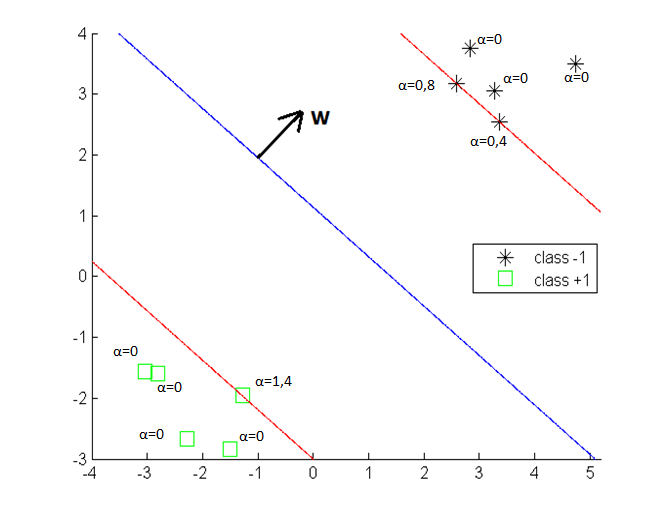
\includegraphics[width=0.6\linewidth]{images/SVM_SV2}
	\caption{Hyperplane obtained after a dual resolution (full blue line). The 2 canonical hyperplanes (red lines) contain the support vectors whose $\alpha_i > 0$. Other points have their $\alpha_i = 0$ and the equation of the hyperplane is only affected by the support vectors.}
	\label{fig:SVM_SV}
\end{figure}


\subsubsection{Kernel trick}
The concept of kernels was introduced by Aizerman \& al. in 1964 to design potential functions in the context of pattern recognition \cite{Aizerman1964}. The idea was re-introduced in 1992 by Boser \& al. for Support Vector Machine ({\sc svm}) and has been received a great number of improvements and extensions to symbolic objects such as text or graphs \cite{Boser1992}.

% One theoretical interesting property of {\sc svm} is that it has been shown that the generalization error bound does not depend on the dimensionality $p$ of the space \cite{Schlkopf2013}. 
From the dual objective in Eq. \ref{eq:dualSVM}, we note that the samples $\textbf{x}_i$ are only involved in a dot-product. Therefore, if we map these samples $\textbf{x}_i$ into a higher dimensional hyperspace, called the feature space, we only need to know the dot product in the feature space:
\begin{equation}
	(\textbf{x}_i . \textbf{x}_j) \rightarrow \Phi(\textbf{x}_i) . \Phi(\textbf{x}_j) 
\end{equation}
\noindent where $\Phi$ is the mapping function. \\

The intuition behind using such mapping is that for many datasets, it is not possible to find a hyperplan that can separate the two classes in the input space if the problem is not linearly separable. However, by applying a transformation $\Phi$, data might become linearly separable in a higher dimensional space. Fig. \ref{fig:SVM_nonlinear} illustrates the idea: in the original 2-dimensional space (left), the two classes can't be separated by a line. However, with a third dimension such that the $+1$ (circle) labeled points are moved forward and the $-1$ (cross) labeled moved back the two classes become separable.

In most of the case, the mapping function $\Phi$ does not need to be known since we only need the dot product $\Phi(\textbf{x}_i) . \Phi(\textbf{x}_j)$. Therefore, we can use any kernel function $\kappa$ such that: $\kappa(\textbf{x}_i,\textbf{x}_j)= \Phi(\textbf{x}_i) . \Phi(\textbf{x}_j)$. We call Gram matrix $G$, the matrix containing all $\kappa(\textbf{x}_i,\textbf{x}_j)$:
\begin{equation*}
	G = (\kappa(\textbf{x}_i,\textbf{x}_j))_{1 \leq i,j \leq n} = 
	\begin{pmatrix}
	\kappa(\textbf{x}_1,\textbf{x}_1) & ... & \kappa(\textbf{x}_1,\textbf{x}_n) \\
	... & & ... \\
	\kappa(\textbf{x}_n,\textbf{x}_1) & ... & \kappa(\textbf{x}_n,\textbf{x}_n) 
	\end{pmatrix}
\end{equation*}

\noindent Defining a kernel has to follow rules. One of these rules specifies that the kernel function has to define a proper inner product in the feature space. Mathematically, the Gram matrix has to be semi-definite positive (Mercer's theorem) \cite{Schlkopf2013}. These restricted feature spaces, containing an inner product are called Hilbert spaces.


\begin{figure}[h!]
\centering
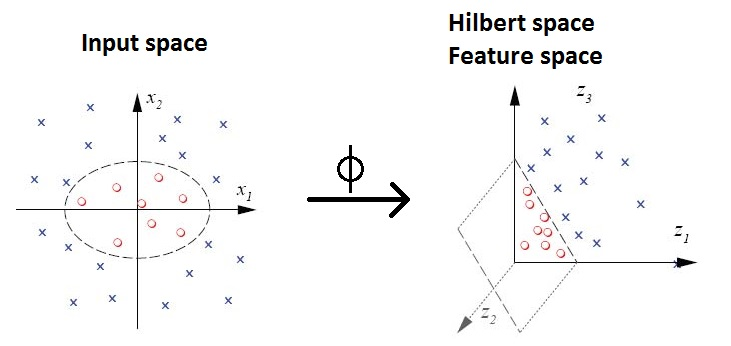
\includegraphics[width=0.9\linewidth]{images/SVM_nonlinear2}
\caption{Left: in two dimensions the two classes of data (-1 for cross and +1 for circle) are mixed together, and it is not possible to separate them by a line: the data is not linearly separable. Right: using a kernel, these two classes of data become separable by a hyperplane in feature space, which maps to the nonlinear boundary shown, back in input space.\protect\footnotemark}
\label{fig:SVM_nonlinear}
\end{figure}
\footnotetext{source: \url{http://users.sussex.ac.uk/~christ/crs/ml/lec08a.html}}

Many kernels have been proposed in the literature such as the polynomial, sigmoid, exponential or wavelet kernels \cite{Schlkopf2013}. The most popular ones that we will use in our work are respectively the Linear and the Gaussian (or Radial Basis Function ({\sc rbf})) kernels:
\begin{align}
	& \kappa(\textbf{x}_i,\textbf{x}_j)= \textbf{x}_i ^T \textbf{x}_j \\
	& \kappa(\textbf{x}_i,\textbf{x}_j)
	= \exp(-\frac{||\textbf{x}_j-\textbf{x}_i||_2^2}{2\sigma^2})
	= \exp(-\gamma||\textbf{x}_j-\textbf{x}_i||_2^2)
\end{align}
where $\gamma = \frac{1}{2\sigma^2}$ is the parameter of the Gaussian kernel and $||\textbf{x}_j-\textbf{x}_i||_2$ is the Euclidean distance between $\textbf{x}_i$ and $\textbf{x}_j$. Note that the Linear kernel is the identity transformation. In practice, for large scale problem (when the number of dimensions $p$ is high), using a Linear kernel is sufficient  \cite{Fan2008}.

The Gaussian kernel computed between a sample $\textbf{x}_j$ and a support vector $\textbf{x}_i$ is an exponentially decaying function in the input space. The maximum value of the kernel ($\kappa(\textbf{x}_i,\textbf{x}_j)$=1) is attained at the support vector (when $\textbf{x}_i=\textbf{x}_j$). Then, the value of the kernel decreases uniformly in all directions around the support vector, with distance and ranges between zero and one. It can thus be interpreted as a similarity measure. Geometrically speaking, it leads to hyper-spherical contours of the kernel function as shown in Fig. \ref{fig:Kernel_Gaussian} \footnote{\url{https://www.quora.com/Support-Vector-Machines/What-is-the-intuition-behind-Gaussian-kernel-in-SVM}}. The parameter $\gamma$ controls the decreasing speed of the sphere. In practice, this parameter is learnt during the training phase.

\begin{figure}[h!]
\centering
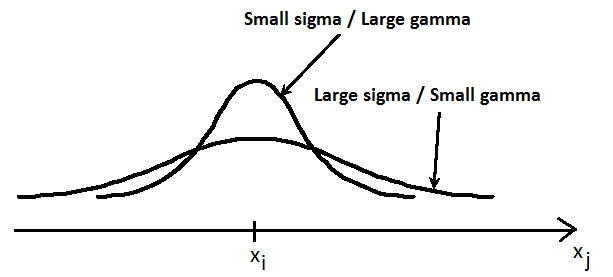
\includegraphics[width=0.6\linewidth]{images/Kernel_Gaussian2}
\caption{Illustration of the Gaussian kernel in the 1-dimensional input space for a small and large $\gamma$ when $\textbf{x}_i$ is fixed and $\textbf{x}_j$ varies.}
\label{fig:Kernel_Gaussian}
\end{figure}


By applying the kernel trick to the soft margin formulation in Eqs. \ref{eq:dualSVM}, \ref{constraintdual1} and \ref{constraintdual4}, the following optimization problem allows to learn non-linear classifiers:
\begin{align}
	& \argmax_{\boldsymbol{\alpha}} \left( 
	\sum\limits_{i=1}^{n} \alpha_i - \frac{1}{2} \sum\limits_{i=1}^{n} \sum\limits_{j=1}^{n} \alpha_i \alpha_j y_i y_j \kappa(\textbf{x}_i , \textbf{x}_j) 
	\right) 
	\label{eq:dualSVM2kernel}\\
	& \textbf{s.t. } \sum\limits_{i=1}^{n}\alpha_i y_i = 0 \label{constraintdual3kernel}\\
	& 0 \leq \alpha_i \leq C  \label{constraintdual4kernel}
\end{align}

\noindent The decision function $f$ becomes:
\begin{equation}
f(\textbf{x}_j) = sign(\sum\limits_{i=1}^{n} \alpha_i^*y_i \kappa(\textbf{x}_i,\textbf{x}_j) + b^*) \label{decisionDualKernel}
\end{equation} 
\noindent Let $n_{SV}$ be the number of support vectors ($n_{SV} \leq n$). To recover $b^*$, we recall that for support vectors $\textbf{x}_i$:
\begin{equation}
	y_j \left( \sum\limits_{i=1}^{n_{SV}} \alpha_i^* y_i \kappa(\textbf{x}_i,\textbf{x}_j) + b^* \right) = 1
\end{equation}
From this, we can solve $b^*$ using an arbitrarily chosen support vector $\textbf{x}_i$:
\begin{equation}
	b^* = \frac{1}{y_j} - \sum\limits_{i=1}^{n_{SV}} \alpha_i^* y_i \kappa(\textbf{x}_i,\textbf{x}_j)
\end{equation}
\noindent Note that in this case, we can't recover the weight vector $\textbf{w}^*$ but it is not useful here for the decision function.

\subsubsection{Interpretation}
\label{subsec:interpretation}
%\begin{itemize}
%	\item interpretation dans le primal: vecteur w et b
%	\item interpretation dans le dual
%	\item interpretation
%\end{itemize}

%\noindent \textbf{Complexity} \\
%\mycomment[CTD]{réécrire + compléter avec Claude}
%As the objective is to provide an algorithm for both small and large datasets, let us examine the complexity of {\sc svm}s and in the computation of the Gram matrix $G$ \cite{Bottou2007}.
%
%In the dual, suppose that we know which samples are not support vectors ($\alpha_i = 0$) and which sample are bounded support vectors ($\alpha_i = C$). The $R$ remaining support vectors are determined by a system of $R$ linear equations. They represent the derivatives of the objective function and requires a number of operations proportional to $R^3$. Verifying that a vector $\alpha$ is a solution of the {\sc svm} problem involves computing the gradient of the dual and checking the optimality conditions. With $n$ samples and $n_{SV}$ support vectors, the number of operations required is equal to $n.n_{SV}$. When $C$ gets large, few support vectors reach the upper bound, the cost is then $R^3 \approx n_{SV}^3$. The term $n.n_{SV}$ is usually larger. The final number of support vectors $n_{SV}$ therefore is the critical component of the computational cost of solving the dual problem. Since the asymptotical number of support vectors $n_{SV}$ grows linearly with the number of samples $n$, the computational cost of solving the {\sc svm} problem has both a quadratic and a cubic component. It grows at least like $n^2$ when $C$ is small and $n^3$ when $C$ gets large.
%
%Computing the $n^2$ components of the kernel matrix $G = \{K(\textbf{x}_i
%, \textbf{x}_j)\}_{i=1}^n$ is a quadratic matter. Note that technical issues may arise in practice. For example, the kernel matrix does not fit in memory when $n$ is large.


\noindent \textbf{Interpretation in the primal} \\
We recall that $\textbf{x}_i$ is a sample in $p$ dimensions: $x_1, \ldots, x_p$. Geometrically, the vector $\textbf{w}$ represents the direction of the hyperplane and points towards the direction of positive decision function $f(\textbf{x}) \geq 0$ (Fig. \ref{fig:SVM_interpretation}). The absolute value of the bias $|b|$ is equal to the distance of the hyperplane to the origin point $\textbf{x}=\textbf{0}$\footnote{$\textbf{0}$ stands for the null vector: $\textbf{0} = [0, \ldots ,0]^T$} if the norm of the vector $\textbf{w}$ is equal to 1. In the soft margin problem, the slack variables $\xi_i$ can be interpreted as follows:
\begin{itemize}
	\item $\xi = 0$ implies that $\textbf{x}_i$ is correctly classified and is either on the margin or on the correct side of the margin.
	\item $0 < \xi \leq 1$ implies that $\textbf{x}_i$ lies inside the margin, but on the correct side of the decision boundary
	\item $\xi \geq 1$ implies that $\textbf{x}_i$ lies on 	the wrong side of the decision boundary and is misclassified.
\end{itemize}
% of the samples $\textbf{x}_i$ that lies within the two canonical hyperplanes are equal to zero. Outside of these canonical hyperplanes, the slack variables $\xi_i > 0$ are equal to the distance to the hyperplane.

\begin{figure}[h!]
	\centering
	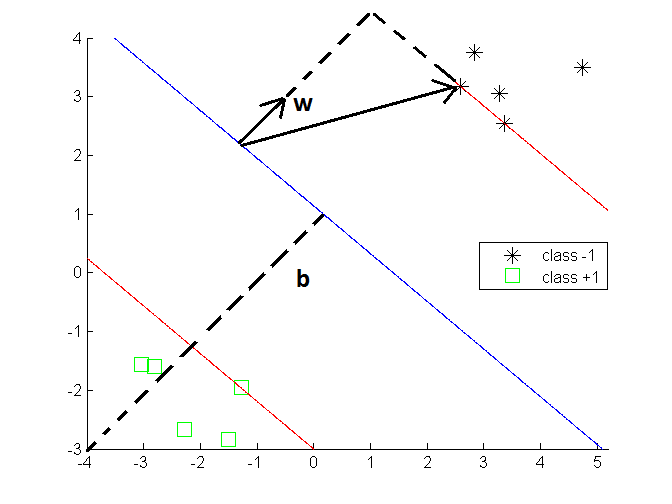
\includegraphics[width=0.7\linewidth]{images/SVM_interpretation2}
	\caption{Geometric representation of SVM.}
	\label{fig:SVM_interpretation}
\end{figure}

In the primal, the weight vector $\textbf{w} = [w_1, \ldots, w_p]^T$ contains as many elements as there are dimensions in the dataset, \textit{i.e.}, $\textbf{w} \in \mathbb{R}^p$. The magnitude of each element in $\textbf{w}$ denotes the importance of the corresponding variable for the classification problem. If the element of $\textbf{w}$ for some variable is 0, these variables are not used for the classification problem.

In order to visualize the above interpretation of the weight vector $\textbf{w}$, let us examine several hyperplanes $\textbf{w}^T\textbf{x}+b=0$ shown in Fig. \ref*{fig:Weight_interpretation} with $p=2$. Fig. \ref{fig:Weight_interpretation}(a) shows a hyperplane where elements of $\textbf{w}$ are the same for both variables $x_1$ and $x_2$. The interpretation is that both variables contribute equally for classification of objects into positive and negative. Fig. \ref{fig:Weight_interpretation}(b) shows a hyperplane where the element of $\textbf{w}$ for $x_1$ is 1, while that for $x_2$ is 0. This is interpreted as that $x_1$ is important but $x_2$ is not. An opposite example is shown in Fig. \ref{fig:Weight_interpretation}(c) where $x_2$ is considered to be important but $x_1$ is not. Finally, Fig. \ref{fig:Weight_interpretation}(d) provides a 3-dimensional example ($p=3$) where an element of $\textbf{w}$ for $x_3$ is 0 and all other elements are equal to 1. The interpretation is that $x_1$ and $x_2$ are important but $x_3$ is not.

\begin{figure}[h!]
	\centering
	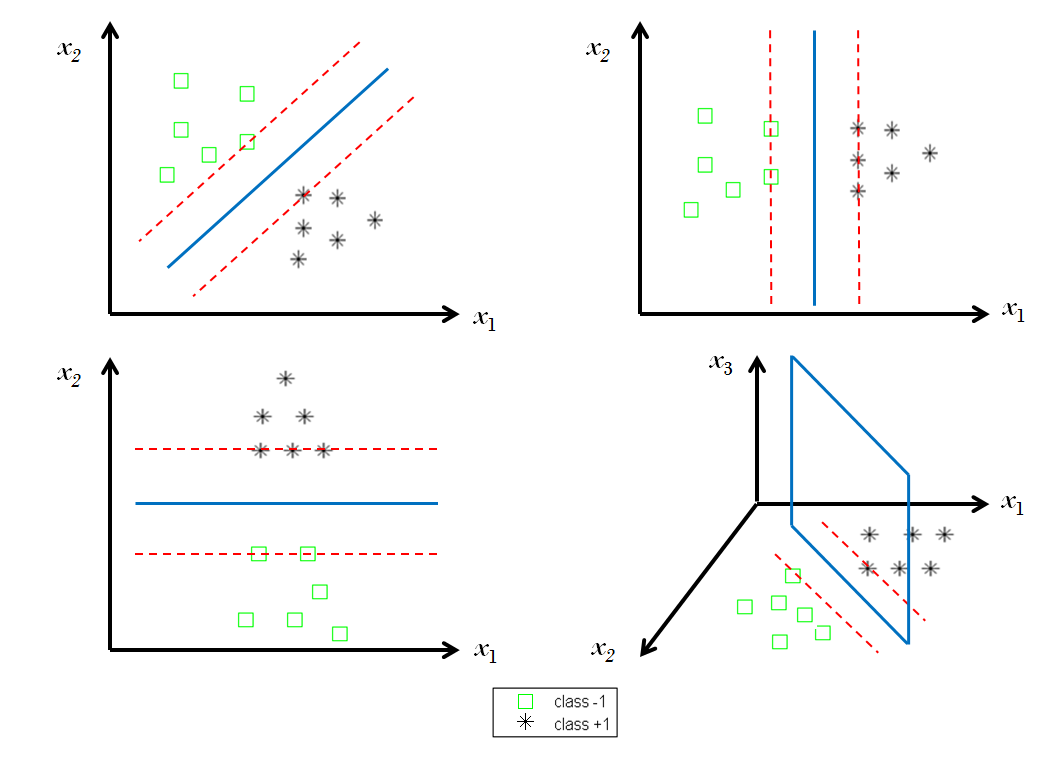
\includegraphics[width=1\linewidth]{Weight_interpretation3}
	\caption{Example of several {\sc svm}s and how to interpret the weight vector $\textbf{w}$}
	\label{fig:Weight_interpretation}
\end{figure}

Another way to interpret how much a variable contributes in the vector $\textbf{w}$ is to express the contribution in percentage: the ratio $\frac{w_j}{||\textbf{w}||_2} . 100$ defines the percentage of contribution for each variable $x_j$ in the {\sc svm} model. The interpretation is only valid if 
the variables $x_j$ of the time series are normalized before learning the {\sc svm} model, they evolves in the same range.



\noindent \textbf{Interpretation in the dual} \\
As a constrained optimization, the dual form satisfies the
Karush-Kuhn-Tucker ({\sc kkt}) conditions (Eqs. \ref{KKT1}, \ref{KKT2} and \ref{KKT3}). We recall Eq. \ref{KKT3}:
\begin{equation*}
	\alpha_i (y_i(\textbf{w}^T\textbf{x}_i+b)-1) = 0
\end{equation*}

From this, for every datapoint $\textbf{x}_i$, either $\alpha_i^* = 0$ or $y_i(\textbf{w}^T\textbf{x}_i+b) = 1$. Any datapoint with $\alpha_i^* = 0$ do not appear in the sum of the decision function $f$ in Eq. \ref{decisionDual} or \ref{decisionDualKernel}. Hence, they play no role for the classification decision of a new sample $\textbf{x}_j$. The others $\textbf{x}_i$ such that $\alpha_i^* > 0$ corresponds to the support vectors. Looking at the distribution of $\alpha_i^*$ allows also to have either a better understanding of the datasets, or either to detect outliers. The higher the coefficient $\alpha_i^*$ for a sample $\textbf{x}_i$ is, the more the sample $\textbf{x}_i$ impacts on the decision function $f$. However, an unusually high value of $\alpha_i^*$ among the samples can lead to two interpretations: either this point is a critical point to the decision, or this point is an outlier. In the soft margin formulation, by constraining $\alpha_i^*$ to be inferior to $C$ (Box constraints) the effect of outliers can be reduced and controlled. 

\subsubsection{Variants of {\sc svm}}
From the primal formulation of {\sc svm} (Eqs. \ref{eq:objectiveSVM} \& \ref{eq:constraintsSVM}), some works investigate the effect of modifications in the regularization and loss term \cite{Hsu2008}.

First, the two common regularizers are $||\textbf{w}||_1$ and $||\textbf{w}||_2$. The former is referred to as $L_1$-Regularizer while the latter is $L_2$-Regularizer. $L_1$-Regularizer is used to obtain sparser models than $L_2$-Regularizer, \textit{i.e.}, the vector $\textbf{w}$ will contain many elements $w_i$ that will equal to zero. Thus, it can be used for variable selection.

Secondly, the two common loss functions $\xi_i$ are $\max(1-y_i \textbf{w}^T \textbf{x}_i, 0)$ and $[\max(1-y_i \textbf{w}^T \textbf{x}_i, 0)]^2$. The former is referred to as $L_1$-Loss and the latter is $L_2$-Loss function. $L_2$-loss function will penalize more slack variables $\xi_i$ during training and would be more sensitive to outliers. Theorically, it should lead to less error in training and poorer generalization in most of the case \cite{Hsu2008}. In general, $L_1$-Loss is preferred.



\subsubsection{Extensions of {\sc svm}}
{\sc svm} has received many interests in recent years. Many extensions has been developed such as $\nu$-{\sc svm}, asymmetric soft margin {\sc svm} or multiclass {\sc svm} \cite{Kijsirikul2002,Crammer2001}. One interesting extension is the extension of Support Vector Machine to regression problems, also called Support Vector Regression ({\sc svr}). The objective is to find a linear regression model $f(\textbf{x})=\textbf{w}^T\textbf{x}+b$. To preserve the property of sparseness, the idea is to consider an $\epsilon$-insensitive error function. It gives zero error if the absolute difference between
the prediction $f(\textbf{x}_i)$ and the target $y_i$ is less than $\epsilon$ where $\epsilon > 0$ penalize samples that are outside of a $\epsilon$-tube as shown as in Fig. \ref{fig:SVR_tube}.

\begin{figure}[h!]
\centering
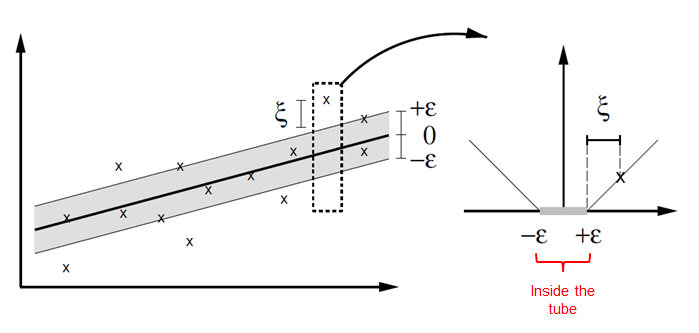
\includegraphics[width=0.8\linewidth]{images/SVR_tube}
\caption{Illustration of {\sc svm} regression (left), showing the regression curve with the $\epsilon$-insensitive "tube" (right). Samples $\textbf{x}_i$ above the $\epsilon$-tube have $\xi_1 > 0$ and $\xi_1 = 0$, points below the $\epsilon$-tube have $\xi_2 = 0$ and $\xi_2 > 0$, and points inside the $\epsilon$-tube have $\xi = 0$.}
\label{fig:SVR_tube}
\end{figure}

\noindent The $\epsilon$-insensitive error function $E_{\epsilon}$ is defined by:
\begin{equation}
E_{\epsilon} (f(\textbf{x}_i)-y_i) =
\left\lbrace
\begin{array}{lll}
0  								& \mbox{if} 		& |f(\textbf{x}_i)-y_i| < \epsilon\\
|f(\textbf{x}_i)-y_i|-\epsilon 	& \mbox{otherwise}  & 
\end{array}\right.
\end{equation}


\noindent The soft margin optimization problem in its primal form is formalized as:
	\begin{align}
		& \argmin_{\textbf{w},b}  \left( 
		\overbrace{\vphantom{\sum_{i=1}^n \xi_i}
			\frac{1}{2}||\textbf{w}||^2_2}^{Regularization}
		+ C \overbrace{\sum\limits_{i=1}^{n}(\xi_{i_1}+\xi_{i_2})}^{Loss}
		\right) 
		\label{eq:objectiveSVR}\\
		& \textbf{s.t. } \forall i=1 \ldots n: \nonumber\\
		& y_i-(\textbf{w}^T\textbf{x}_i+b) \geq \epsilon -\xi_{i_1} \\
		& (\textbf{w}^T\textbf{x}_i+b)-y_i \geq \epsilon -\xi_{i_2} \\
		&  \xi_{i_1} \geq 0 \\
		&  \xi_{i_2} \geq 0
	\end{align}

\noindent The slack variables are divided into 2 kind of slacks variables, one for samples above the decision function $f$ ($\xi_{i_1}$), and one for samples under the decision function $f$ ($\xi_{i_2}$). As for {\sc svm}, it is possible to have a dual formulation:
	\begin{align}
		& \argmax_{\boldsymbol{\alpha}} 
		\left( 
		\sum\limits_{i=1}^{n} y_i(\alpha_{i_1}-\alpha_{i_2})
		-\frac{1}{2} \sum\limits_{i=1}^{n} \sum\limits_{j=1}^{n} (\alpha_{i_1}-\alpha_{i_2})(\alpha_{j_1}-\alpha_{j_2}) (\textbf{x}_i.\textbf{x}_j)
		\right) \\ 
		& \textbf{s.t. } \forall i=1 \ldots n: \nonumber\\
		& \sum\limits_{i=1}^{n} \alpha_{i_1} = \sum\limits_{i=1}^{n} \alpha_{i_2} \\
		& 0 \leq \alpha_{i_1} \leq C \\
		& 0 \leq \alpha_{i_2} \leq C
	\end{align}
\noindent As in {\sc svm}, we obtain three possible regression functions for a new sample $\textbf{x}_j$, respectively in its primal, dual, and non-linear form:
\begin{align}
	& f(\textbf{x}_j) = \textbf{w}^T\textbf{x}_j+b \\ 
	& f(\textbf{x}_j) = \sum\limits_{i=1}^{n} (\alpha_{i_1}^*-\alpha_{i_2}^*)(\textbf{x}_i.\textbf{x}_j) + b \\	
	& f(\textbf{x}_j) = \sum\limits_{i=1}^{n} (\alpha_{i_1}^*-\alpha_{i_2}^*)K(\textbf{x}_i,\textbf{x}_j) + b
\end{align}	
More informations about the calculation development can be found in \cite{Bishop2006}.

\subsection{Other classification algorithms}
\todo[inline]{Partie non encore rédigée. A faire à la fin.}
\begin{itemize}
	\item Positionner les travaux par rapport aux autres méthodes d'apprentissage supervisé
	\item S'intéresser au Deep neural network (à la mode en ce moment)
	\item RVM, Decision Tree, 
	\item Ne pas trop développer
	\item Dans notre cas, on ne s'intéressera pas à ce type d'algorithmes (type deep learning) car il ne repose pas sur une notion de distance et les features qui sont trouvés ne sont pas interprétables
\end{itemize}



%----------------------------------------------------------------------------
\section{Conclusion of the chapter}
%\begin{itemize}
%	\item The concept of order of temporal data in not take into account (dynamic, frequence, etc.)
%	\item Introduction to next chapter: all of these algorithms (kNN, {\sc svm}, etc.) are based on a notion of distance or similarity between objects to compare/classify. Let consider now the object time series and let recall the concept of distance between time series
%\end{itemize}
\todo[inline]{A refaire complètement à la fin.}
This chapter reviews the different steps in a machine learning framework: data normalization, model selection and model evaluation. We focus on two machine learning algorithms used in our proposition: the $k$-Nearest Neighbors ($k$-NN) and the Support Vector Machine ({\sc svm}). In the following, we consider the $k$-NN as our classifier. The {\sc svm} will be used in our work for its large margin concept. 

Our objective being the learning of a metric that optimizes the performances of the $k$-NN classifier, we review in the next section some metrics proposed for time series as well as metric learning concept for static data.

%To make the classification or regression of time series, a commonly hypothesis is to consider time series as static data and then to apply classical machine learning algorithms, such as a $k$-Nearest Neighbors ($k$-NN) or a Support Vector Machine ({\sc svm}) approach. For that, the practitioner has to be careful on the design of his learning framework: data must be separated into a training and testing set, data have to be normalized depending on their distributions, cross-validation must be operated on the training set to learn the best fitting of the hyper-parameters and finally, performance metrics and statistical tests should be used to compare the performances of different classifiers.
%
%In the following, we consider the $k$-NN as our classifier. The {\sc svm} will be used in our work for its generalization properties thanks to the large margin concept. A key aspect in $k$-NN relies on the comparison of time series through metrics. Assuming that time series can be reduced to flat data may be too restrictive. Under such hypothesis and using a standard Euclidean distance, time series are only compared on their amplitude at the same time. However, time series are more complex. They may exhibit similar behavior or share similar frequential spectrum. Thus, there is a need to consider time series as an ordered object and to define adapted metrics for time series.


%%% Local Variables: 
%%% mode: latex
%%% TeX-master: "../roque-phdthesis"
%%% End: 
